\documentclass[10pt]{beamer}
\usetheme{Madrid}
\usepackage[utf8]{inputenc}
\usepackage[T1]{fontenc}
\usepackage{lmodern}
\usepackage[polish]{babel}
\usepackage{booktabs}
\usepackage{hyperref}
\usepackage{graphicx}

\title{Wykrywanie fake news}
\subtitle{Porównanie modeli językowych na zbiorze LIAR}
\date{Czerwiec 2026}

\begin{document}

\maketitle

\section{Problem i dane}

\begin{frame}{Cel projektu}
  Klasyfikacja prawdziwości wypowiedzi politycznych na \textbf{zbiorze LIAR}.

  \vspace{0.5em}
  Dwa warianty zadania:
  \begin{itemize}
    \item \textbf{Binarna (2kl)}: \texttt{fake} / \texttt{real}
    \item \textbf{Sześcioklasowa (6kl)}: \texttt{pants-fire}, \texttt{false},
          \texttt{barely-true}, \texttt{half-true}, \texttt{mostly-true}, \texttt{true}
  \end{itemize}

  \vspace{0.5em}
  Porównujemy dwa paradygmaty:
  \begin{enumerate}
    \item \textbf{Fine-tuning encodera} -- BERT-base, RoBERTa-base, RoBERTa-large
    \item \textbf{Prompting LLM} -- GPT-4o-mini, GPT-4o; darmowe (OpenRouter):
          gpt-oss-20b, gemma-4-31b-it, dolphin-mistral-24b, llama-3.3-70b-instruct
  \end{enumerate}
\end{frame}

\begin{frame}{Zbiór LIAR}
  \small
  \begin{itemize}
    \item 12 791 wypowiedzi z PolitiFact (train 10 240 / val 1 284 / test 1 267)
    \item Treść + mówca, partia, temat, historia prawdziwości
    \item Tematy: gospodarka, zdrowie, podatki, edukacja, wybory, imigracja
    \item Granice między 6 klasami są subiektywne -- nawet sami fact-checkerzy
          z PolitiFact często nie są zgodni przy przypisywaniu wypowiedzi do
          jednej z sześciu etykiet
  \end{itemize}

  \vspace{0.5em}
  \scriptsize
  \begin{center}
  \begin{tabular}{lp{6cm}}
    \toprule
    Zbiór & Co zawiera \\
    \midrule
    \textbf{LIAR}      & treść + metadane mówcy \\
    \textbf{LIAR-PLUS} & LIAR + \texttt{justification} (uzasadnienie fact-checkera) \\
    LIAR2              & rozszerzona wersja (~22k wypowiedzi, 2024) \\
    LIAR-RAW           & surowe dane scrapowane z PolitiFact \\
    \bottomrule
  \end{tabular}
  \end{center}
\end{frame}

\begin{frame}{Rozkład klas w zbiorze LIAR}
  \begin{center}
    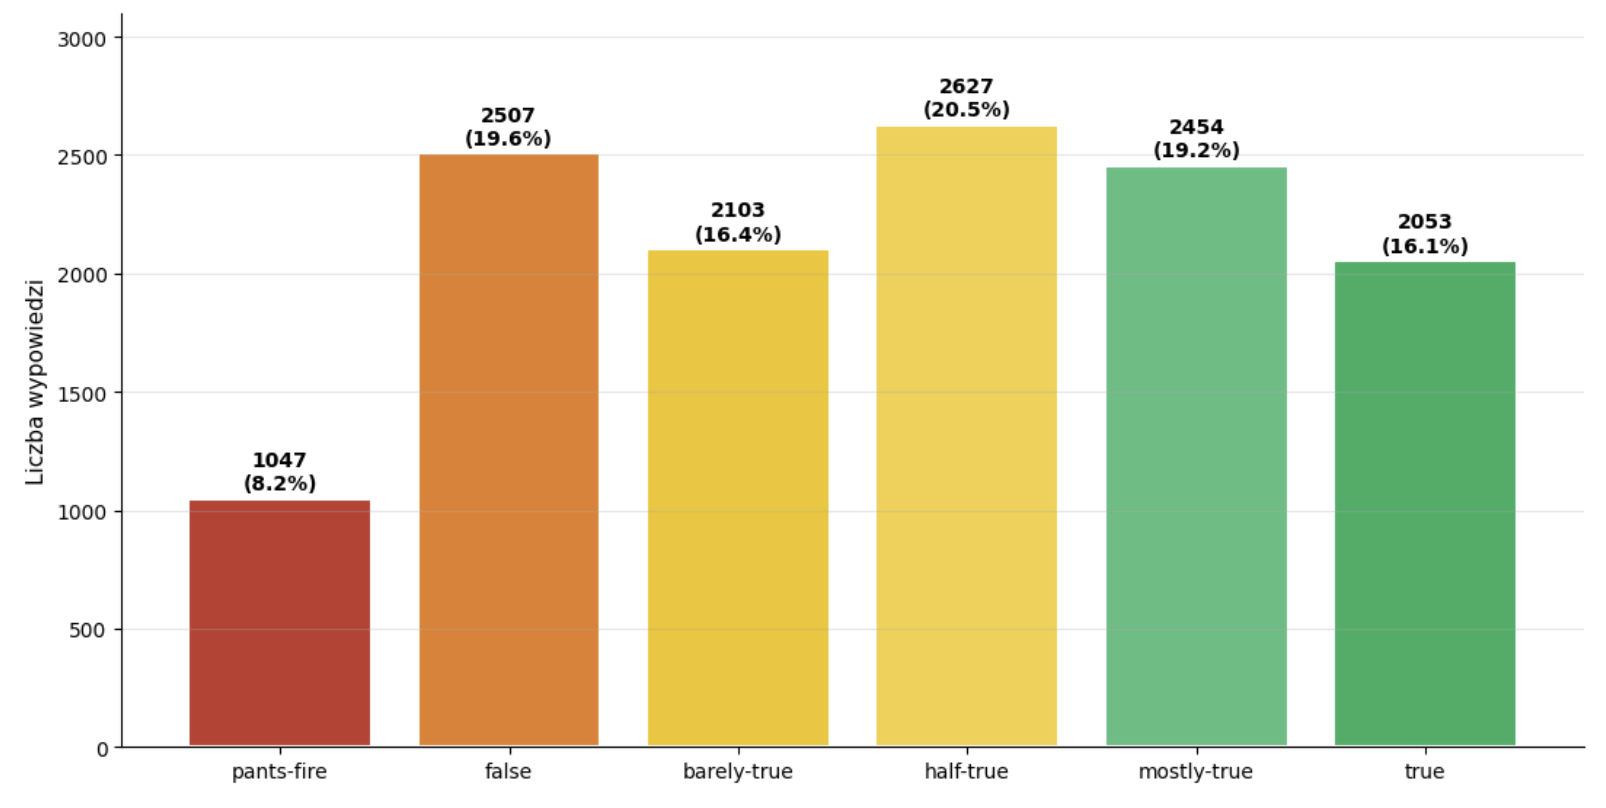
\includegraphics[width=0.95\textwidth]{label_distribution.png}
  \end{center}
\end{frame}

\begin{frame}{Struktura zbioru LIAR}
  \small
  Każda wypowiedź ma 14 kolumn:
  \begin{center}
  \begin{tabular}{ll}
    \toprule
    Kolumna & Znaczenie \\
    \midrule
    \texttt{id}                 & unikalny identyfikator wypowiedzi \\
    \texttt{label}              & etykieta (\texttt{pants-fire} ... \texttt{true}) \\
    \texttt{statement}          & treść wypowiedzi (główny tekst) \\
    \texttt{subject}            & temat (np. economy, education) \\
    \texttt{speaker}            & mówca \\
    \texttt{job\_title}         & stanowisko mówcy \\
    \texttt{state}              & stan USA \\
    \texttt{party}              & partia polityczna \\
    \texttt{barely\_true\_counts} & liczba poprzednich \texttt{barely-true} \\
    \texttt{false\_counts}      & liczba poprzednich \texttt{false} \\
    \texttt{half\_true\_counts} & liczba poprzednich \texttt{half-true} \\
    \texttt{mostly\_true\_counts} & liczba poprzednich \texttt{mostly-true} \\
    \texttt{pants\_on\_fire\_counts} & liczba poprzednich \texttt{pants-fire} \\
    \texttt{context}            & kontekst (np. campaign rally, interview) \\
    \bottomrule
  \end{tabular}
  \end{center}

  \vspace{0.3em}
  Kolumny \texttt{*\_counts} to \emph{credit history} -- wiarygodność mówcy
  na podstawie historii.
\end{frame}

\begin{frame}{Preprocessing}
  Każda wypowiedź łączona w jeden tekst:
  \begin{quote}\small
    \texttt{\{speaker\} (\{party\}, past lies: N, past truths: M):\\
    \{statement\} Subject: \{subject\} Context: \{context\}}
  \end{quote}

  \begin{itemize}
    \item Mapowanie etykiet 6kl $\to$ 2kl (\emph{tylko dla modeli dwuklasowych}):
          \texttt{pants-fire/false/barely-true} $\to$ \texttt{fake},\\
          \texttt{half-true/mostly-true/true} $\to$ \texttt{real}
    \item 99{,}96\% wypowiedzi mieści się w 128 tokenach (mediana = 22) --
          stąd \texttt{max\_length=128} w tokenizacji
    \item Tokenizacja \texttt{AutoTokenizer}: BPE dla RoBERTy, WordPiece dla BERT-a
    \item Wagi klas: $w_c = N/(C \cdot n_c)$
          przeciwdziałają niezbalansowaniu
    \item Tensory \texttt{input\_ids}, \texttt{attention\_mask}, \texttt{labels}
          opakowane w \texttt{DataLoader}
  \end{itemize}
\end{frame}

\begin{frame}{Performance Ceiling -- wyniki z literatury}
  \scriptsize
  \begin{columns}[T]
    \begin{column}{0.5\textwidth}
      \centering
      \textbf{Wang 2017 -- oryginalny paper LIAR (6kl)}\\[2pt]
      \begin{tabular}{lrr}
        \toprule
        Models               & Valid. & Test \\
        \midrule
        Majority             & 0{,}204 & 0{,}208 \\
        SVMs                 & 0{,}258 & 0{,}255 \\
        Logistic Regression  & 0{,}257 & 0{,}247 \\
        Bi-LSTMs             & 0{,}223 & 0{,}233 \\
        CNNs                 & 0{,}260 & 0{,}270 \\
        \midrule
        \multicolumn{3}{l}{Hybrid CNNs} \\
        Text + Subject       & 0{,}263 & 0{,}235 \\
        Text + Speaker       & \textbf{0{,}277} & 0{,}248 \\
        Text + Job           & 0{,}270 & 0{,}258 \\
        Text + State         & 0{,}246 & 0{,}256 \\
        Text + Party         & 0{,}259 & 0{,}248 \\
        Text + Context       & 0{,}251 & 0{,}243 \\
        Text + History       & 0{,}246 & 0{,}241 \\
        Text + All           & 0{,}247 & \textbf{0{,}274} \\
        \bottomrule
      \end{tabular}\\[2pt]
      {\tiny Źródło: Wang (ACL 2017)}
    \end{column}

    \begin{column}{0.5\textwidth}
      \centering
      \begin{tabular}{lrr}
        \toprule
        Model & Test Acc & W-F1 \\
        \midrule
        Linear SVM (BoW) -- 2kl                  & 0{,}624 & 0{,}316 \\
        RoBERTa (prior) -- 2kl                   & 0{,}620 & -- \\
        XGBoost (GloVe, overfit) -- 6kl          & 0{,}249 & -- \\
        GPT-3 Curie (fine-tuned) -- 6kl          & 0{,}295 & -- \\
        \bottomrule
      \end{tabular}\\[2pt]
      {\tiny Źródło: emergentmind.com/topics/liar-benchmark}

    \end{column}
  \end{columns}
\end{frame}

\section{Metody}

\begin{frame}{BERT vs RoBERTa}
  \small
  \textbf{RoBERTa} (Robustly Optimized BERT, Liu et al.\ 2019) -- model
  językowy typu \emph{encoder-only}, oparty na architekturze Transformer.
  Czyta tekst dwukierunkowo i produkuje gęsty wektor reprezentacji,
  idealny do klasyfikacji (nie generuje tekstu).

  \emph{Mechanizm attention:} dla każdego słowa model uczy się jakie
  \emph{wagi} przypisać innym słowom w zdaniu -- w jednym przejściu
  każdy token może spojrzeć na każdy inny, dzięki czemu model uchwyca
  długie zależności kontekstowe.

  \vspace{0.3em}
  \textbf{RoBERTa vs BERT:}
  \begin{center}
  \begin{tabular}{lll}
    \toprule
     & \textbf{BERT (Devlin 2019)} & \textbf{RoBERTa (Liu 2019)} \\
    \midrule
    Korpus pretreningu & 16 GB (Wiki+Books) & \textbf{160 GB} (+CC-News, OpenWebText) \\
    Maskowanie         & statyczne          & \textbf{dynamiczne} \\
    Zadanie pretrenu   & MLM + NSP          & \textbf{tylko MLM} (NSP nie pomaga) \\
    Batch size         & 256                & \textbf{8K} \\
    \bottomrule
  \end{tabular}
  \end{center}

  \vspace{0.3em}
  \scriptsize
  \textbf{Testujemy obie wersje -- \texttt{roberta-base} i \texttt{roberta-large}:}
  \begin{itemize}
    \item \texttt{roberta-base} (125M par., 12 warstw, hidden 768) -- mniejszy,
          szybszy do trenowania
    \item \texttt{roberta-large} (355M par., 24 warstwy, hidden 1024) --
          spodziewamy się wyższych wyników kosztem dłuższego treningu
  \end{itemize}
\end{frame}

\begin{frame}{Metryki ewaluacji}
  \small
  \textbf{Stosowane metryki:}
  \begin{itemize}
    \item \textbf{accuracy} -- udział poprawnych predykcji
    \item \textbf{precision}, \textbf{recall} per klasa (oraz średnie macro / weighted)
    \item \textbf{F1} per klasa -- $F_1 = \dfrac{2 \cdot \text{precision} \cdot \text{recall}}{\text{precision} + \text{recall}}$
    \item \textbf{weighted-F1} -- średnia F1 ważona supportem klas
    \item \textbf{\underline{macro-F1}} -- nasza główna metryka:
    \[
      \text{macro-F1} = \frac{1}{C} \sum_{c=1}^{C} F_1^{(c)}
    \]
    średnia arytmetyczna F1 z każdej klasy, bez ważenia liczebnością --
    traktuje każdą klasę jednakowo i karze model za ignorowanie klas rzadkich,
    kluczowych w fact-checkingu (np. \texttt{pants-fire})
    \item \textbf{ROC AUC} (one-vs-rest) -- jak dobrze model rankuje klasy
    \item \textbf{macierz pomyłek} -- które klasy mylą się ze sobą
  \end{itemize}
\end{frame}

\begin{frame}{Techniki podnoszące jakość}
  \begin{itemize}
    \item \textbf{Wagi klas} (Cross-Entropy z $w_c = N/(C \cdot n_c)$)
    \item \textbf{Label smoothing} ($\varepsilon = 0{,}1$)
    \item \textbf{Optuna} -- 20 triali, TPE sampler, MedianPruner
    \item \textbf{Early stopping} po val macro-F1
    \item \textbf{Linear warmup + decay} schedulera lr
    \item \textbf{Structured Outputs} (GPT) -- JSON schema, 0 unparsed
    \item \textbf{Self-consistency} (GPT) -- N=3 niezależne predykcje + voting
    \item \textbf{Few-shot kNN retrieval} -- TF-IDF cosine similarity
  \end{itemize}

\end{frame}

\begin{frame}{Optuna -- automatyczne strojenie hiperparametrów}
  \begin{columns}[T]
    \begin{column}{0.55\textwidth}
      \small
      \textbf{Co to:} framework do automatycznego wyszukiwania
      hiperparametrów.

      \begin{itemize}
        \item \textbf{TPE Sampler} -- Bayesowski wybór kolejnych prób,
              uczy się z wcześniejszych
        \item \textbf{MedianPruner} -- ucina słabe triale po E1
              (poniżej mediany), oszczędza GPU
      \end{itemize}

      \textbf{Uzasadnienie użycia:} 50 kombinacji ręcznie = dni GPU; Optuna 20 prób = 2h.

      \textbf{Efekt:} val F1 $0{,}71 \to \textbf{0{,}7435}$ (+3 pkt).

      \vspace{0.3em}
      \scriptsize
      Best params z 2kl stosujemy też do treningu 6kl (i 6kl + LIAR-PLUS),
      czasem z ręcznym dopasowaniem (\texttt{epochs}, \texttt{weight\_decay})
      pod większą trudność zadania.
    \end{column}
    \begin{column}{0.45\textwidth}
      \small
      \centering
      \textbf{Best params (2kl):}
      \vspace{0.3em}
      \begin{tabular}{lr}
        \toprule
        parametr & wartość \\
        \midrule
        learning rate & $5{,}79 \cdot 10^{-6}$ \\
        weight decay  & $0{,}124$ \\
        epochs        & 5 \\
        batch size    & 8 \\
        \midrule
        \textbf{val F1} & \textbf{0{,}7435} \\
        \bottomrule
      \end{tabular}
    \end{column}
  \end{columns}
\end{frame}

\section{Wyniki}

\begin{frame}{Wyniki -- GPT (OpenAI API) + darmowe LLM}
  \scriptsize
  \begin{center}
  \begin{tabular}{lrrrr}
    \toprule
    Model & 2kl Acc & 2kl Macro-F1 & 6kl Acc & 6kl Macro-F1 \\
    \midrule
    \multicolumn{5}{l}{\textbf{OpenRouter (darmowe)} \emph{-- w trakcie ewaluacji}} \\
    gpt-oss-20b (ZS)                     & 0{,}467 & 0{,}407 & --- & --- \\
    gemma-4-31b-it                       & --- & --- & --- & --- \\
    dolphin-mistral-24b                  & --- & --- & --- & --- \\
    llama-3.3-70b-instruct               & --- & --- & --- & --- \\
    \midrule
    \multicolumn{5}{l}{\textbf{GPT (OpenAI, płatne)}} \\
    GPT-4o-mini zero-shot                & 0{,}696 & 0{,}695 & 0{,}298 & 0{,}279 \\
    GPT-4o-mini few-shot                 & 0{,}693 & 0{,}686 & 0{,}324 & 0{,}310 \\
    GPT-4o zero-shot (SC=3, SO)          & \textbf{0{,}729} & \textbf{0{,}729} & --- & --- \\
    GPT-4o few-shot                      & 0{,}710 & 0{,}709 & \textbf{0{,}344} & \textbf{0{,}356} \\
    \bottomrule
  \end{tabular}
  \end{center}
\end{frame}

\begin{frame}{Wyniki -- fine-tuning encoderów}
  \small
  \begin{center}
  \begin{tabular}{lrrrr}
    \toprule
    Model & 2kl Acc & 2kl Macro-F1 & 6kl Acc & 6kl Macro-F1 \\
    \midrule
    BERT-base-uncased                    & 0{,}628 & 0{,}604 & --- & --- \\
    RoBERTa-base                         & 0{,}640 & 0{,}622 & --- & --- \\
    \textbf{RoBERTa-large baseline}      & \textbf{0{,}738} & \textbf{0{,}728} & --- & --- \\
    RoBERTa-large + Optuna               & --- & --- & 0{,}357 & 0{,}359 \\
    RoBERTa-large + LIAR-PLUS            & --- & --- & 0{,}355 & 0{,}341 \\
    \bottomrule
  \end{tabular}
  \end{center}

\end{frame}

\begin{frame}{LLM prompting -- techniki GPT}
  \begin{itemize}
    \item \textbf{Structured Outputs} -- każemy modelowi odpowiadać
          tylko jednym słowem (\texttt{fake} lub \texttt{true}),
          zero zbędnego tekstu
    \item \textbf{Few-shot kNN} -- wklejamy do promptu kilka
          przykładów ze zbioru treningowego najbardziej podobnych
          do pytanego zdania
    \item \textbf{Self-consistency} -- pytamy model 3 razy,
          bierzemy odpowiedź, która padła najczęściej
  \end{itemize}
\end{frame}

\begin{frame}{Najlepsze wyniki z każdej kategorii}
  \small
  \begin{center}
  \begin{tabular}{llcc}
    \toprule
    Kategoria & Model & 2kl Macro-F1 & 6kl Macro-F1 \\
    \midrule
    Encoder (fine-tune) & RoBERTa-large (+ LIAR-PLUS na 6kl) & \textbf{0{,}728} & 0{,}341 \\
    LLM płatny (API)    & gpt-4o (SC=3, SO / few-shot)       & 0{,}729          & 0{,}356 \\
    \bottomrule
  \end{tabular}
  \end{center}

  \vspace{0.5em}
  \begin{itemize}
    \item 2kl: \textbf{remis} -- RoBERTa-large $\approx$ gpt-4o (0{,}728 vs 0{,}729)
    \item 6kl: \textbf{GPT-4o} (0{,}356) nieznacznie wyprzedza RoBERTa-large + LIAR-PLUS (0{,}341)
  \end{itemize}
\end{frame}

\begin{frame}{Czas wykonania}
  \small
  \begin{center}
  \begin{tabular}{lrr}
    \toprule
    Eksperyment & Czas & Per próbka \\
    \midrule
    \multicolumn{3}{l}{\textbf{GPT-4o-mini (API)} -- 1267 próbek} \\
    2kl zero-shot           & 94 s     & 75 ms \\
    2kl few-shot            & 163 s    & 130 ms \\
    6kl zero-shot           & 714 s ($\sim$12 min) & 560 ms \\
    6kl few-shot            & 4001 s ($\sim$67 min) & 3{,}2 s \\
    \midrule
    \multicolumn{3}{l}{\textbf{GPT-4o (API, próba 2)}} \\
    2kl zero-shot SC=3      & 160 s    & 125 ms \\
    6kl few-shot K=1 SC=1   & 2007 s ($\sim$33 min) & 1{,}6 s \\
    \midrule
    \multicolumn{3}{l}{\textbf{RoBERTa-large (A100, trening + ewaluacja)}} \\
    2kl trening 5 epok      & $\sim$10 min & --- \\
    Optuna 2kl (20 triali)  & $\sim$2 h    & --- \\
    6kl\_plus 7 epok        & $\sim$25 min & --- \\
    \bottomrule
  \end{tabular}
  \end{center}
\end{frame}

\section{Wnioski}

\begin{frame}{Wnioski}
  \begin{itemize}
    \item \textbf{Fine-tuning vs prompting:}
          \begin{itemize}
            \item 2kl: RoBERTa-large $\geq$ GPT-4o (lokalnie, 0$\$$ inferencji)
            \item 6kl: GPT-4o $\geq$ RoBERTa (wiedza o świecie)
            \item RoBERTa-large + LIAR-PLUS -- nasze najlepsze 6kl
          \end{itemize}
    \item \textbf{Few-shot nie pomaga} w fact-checkingu -- przykłady
          uczą modelu \emph{formatu odpowiedzi}, ale nie dostarczają wiedzy
          potrzebnej do oceny prawdziwości nowej, niezwiązanej wypowiedzi
          (prawdziwość zależy od faktów o świecie, nie od wzorca)
    \item \textbf{Structured Outputs} -- musi być (z 11\% unparsed do 0\%)
    \item \textbf{Macro-F1, nie accuracy} -- niezbalansowane klasy
    \item \textbf{Performance ceiling 6kl} ($\sim$0{,}32) przekroczyliśmy dzięki LIAR-PLUS
  \end{itemize}
\end{frame}

\end{document}
